\documentclass[tikz,border=10pt]{standalone}
\begin{document}
	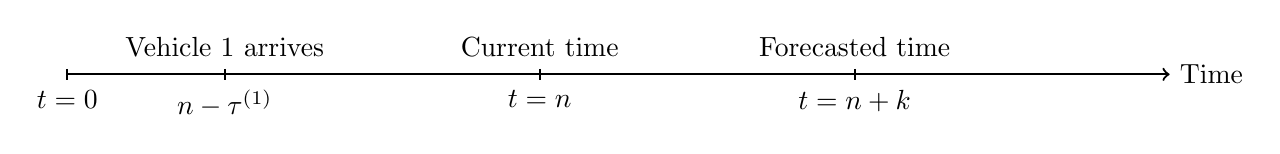
\begin{tikzpicture}[thick, scale=1]
		% Draw the timeline
		\draw[->] (0,0) -- (14,0) node[right] {Time};
		
		% Mark the time points
		\foreach \x/\label in {0/$t=0$, 2/$n-\tau^{(1)}$, 6/$t=n$, 10/$t=n+k$} {
			\draw (\x,2pt) -- (\x,-2pt) node[below] {\label};
		}

		% Add annotations
		\node[above] at (2, 0.1) {Vehicle 1 arrives};
		\node[above] at (6, 0.1) {Current time};
		\node[above] at (10, 0.1) {Forecasted time};
	\end{tikzpicture}
\end{document}
